\section{Language Modeling}
\label{chap:Language Modeling}

  %%%%%%%%%%%%%%%%%%%%%%%%%%%%
  % SUBSECTION               %
  %%%%%%%%%%%%%%%%%%%%%%%%%%%%
\subsection{Introduction}
Formal languages, like programming languages, can be fully specified.
All the reserved words can be defined and the valid ways that they can be used can be precisely defined.
We cannot do this with natural language. Natural languages are not designed; they emerge, and therefore there is no formal specification.\\
Further, languages change, word usages change; it is a moving target.Nevertheless, linguists try to specify the language with formal grammars and structures. It can be done, but it is very difficult and the results can be fragile.
An alternative approach to specifying the model of the language is to learn it from examples.\cite{web012}
\subsection{Statistical Language Modeling}
Language modeling is the development of probabilistic models that are able to predict the next word in the sequence given the words that precede it. LM is the task of assigning a probability to sentences in a language. Besides assigning a probability to each sequence of words, the language models also assigns a probability for the likelihood of a given word (or a sequence of words) to follow a sequence of words. \\A language model learns the probability of word occurrence based on examples of text. Simpler models may look at a context of a short sequence of words, whereas larger models may work at the level of sentences or paragraphs. Most commonly, language models operate at the level of words.\\
Language models are used to generate text in many similar natural language processing tasks, for example:Optical Character Recognition (OCR), Handwriting Recognition, Spelling Correction, Machine Translation, automated QA ... etc.
\subsection{Neural Language Models}
The use of neural networks in language modeling is often called Neural Language Modeling, or NLM for short. Recently, the use of neural networks in the development of language models has become very popular, to the point that it may now be the preferred approach. Neural network approaches are achieving better results than classical methods both on standalone language models and when models are incorporated into larger models on challenging tasks like speech recognition and machine translation or even QA.\\Specifically, a word embedding is adopted that uses a real-valued vector to represent each word in a project vector space.  This learned representation of words based on their usage allows words with a similar meaning to have a similar representation.\subsubsection{Word Embeddings}Neural Language Models (NLM) address the n-gram data sparsity issue through parameterization of words as vectors (word embeddings) and using them as inputs to a neural network. The parameters are learned as part of the training process. Word embeddings obtained through NLMs exhibit the property whereby semantically close words are likewise close in the induced vector space. “True generalization” is difficult to obtain in a discrete word indice space, since there is no obvious relation between the word indices.\\Character-level Convolutional Neural Network (CNN) models can be used on the front-end instead of word embeddings, achieving similar and sometimes better results.\subsubsection{Neural Network Approach to Language Modeling}The neural network approach to language modeling can be described using the three following model properties: \\ \indent$\bullet$Associate each word in the vocabulary with a distributed word feature vector.\\\indent$\bullet$Express the joint probability function of word sequences in terms of the feature vectors of these words in the sequence.\\
\indent$\bullet$Learn simultaneously the word feature vector and the parameters of the probability function.\\
 Recurrent neural networks and then networks with a long-term memory like the Long Short-Term Memory (LSTM), or GRU, allow the models to learn the relevant context over much longer input sequences than the simpler feed-forward networks.
 \subsection{NLM in TensorFlow}
 \subsubsection{WHY Tensorflow ?}  
Tensorflow Known as the second-generation machine learning system, it performs numerical computations through data flow graphs. Mathematical computations with a directed graph involves nodes and edges; nodes implement mathematical operations and can also show endpoints to feed in data, deliver outcome/ read/write persistent variables, whereas the edges explain the input/output relationships between nodes. 
 \subsubsection{Using a Dynamic RNN}
 Static construction of RNN adds every node for every timestep to the graph before execution. Tensorflow allows us to create the graph at runtime to speed things up. So dynamically create the graph at execution time, which can be more efficient.\\
 To do this, instead of using a list of tensors (of length \texttt{num\_steps} and shape  [\texttt{batch\_size}, features]), we keep everything in a single 3-dimnesional tensor of shape  [\texttt{batch\_size}, \texttt{num\_steps}, features], and use Tensorflow’s dynamic rnn function.\cite{web013}
   \begin{figure}[H]%
    \center%
    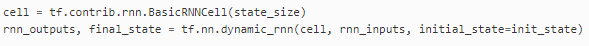
\includegraphics[width=\textwidth]{images/amir/dy_rnn.png}%
     % you need to add the caption for the list of figures
    \caption[This is a dynamic rnn code image]{\texttt{dynamic\_rnn} code}\label{fig:dynamic rnn}%
  \end{figure}
\subsection{Unrolling RNN}
Unrolling can speed-up a RNN, although it tends to be more memory-intensive. Unrolling is only suitable for short sequences in generating sequences of words or chars.
RNNs are fit and make predictions over many time steps. We can simplify the model by unfolding or unrolling the RNN graph over the input sequence. Also, this “full unrolling” makes a parallel training with multiple sequences inefficient on shared memory models such as graphics processing units (GPUs).\cite{web014} Unrolling of the forward pass when the network is copied for each input time step. Unrolling of the backward pass for updating network weights during training.
  \begin{figure}[H]%
    \center%
    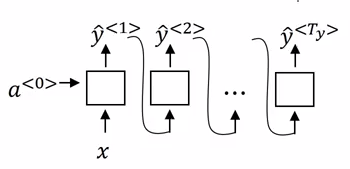
\includegraphics[width=\textwidth]{images/amir/unroll_rnn.png}
     % you need to add the caption for the list of figures
    \caption[This is a unrolling rnn image]{unrolling rnn for generating sequence}\label{fig:unrolling rnn}%
  \end{figure}